W celu przeprowadzenia badania nad wydajnością oraz porównaniem trzech różnych aplikacji serwujących podobne API, zdecydowano się na implementację trzech aplikacji w różnych technologiach: Django, .NET oraz NestJS.
Każda z aplikacji została skonfigurowana do korzystania z bazy danych PostgreSQL. Schemat środowiska badawczego został na rysunku \ref{rys:docker_schema}.
Całe środowisko, a więc aplikacja oraz baza danych, zostało uruchomione w kontenerach Docker w lokalnym środowisku.
Część zbierania danych została oddzielona od samego opracowywania wyników.
Grafana K6 zapisywał pliki z wynikami, które następnie były konsumowane przez skrypt opracowyjący wyniki.
Skrypty zostały napisane w Jupiter Notebook, które pozwala uruchamiać skrypty systemowe oraz w języku python w ramach arkusza.
Zaletą tego rozwiązania jest zapisany nie tylko skrypt ale również częściowy wynik programu w przystępny sposób.
Dowolny fragment arkusz może zostać uruchmiony powtórnie.
Jest to również dogodne środowisko do przeglądania danych oraz ich rysowania.
Kroki badania zostały zaprezentowane na rysunku \ref{rys:test_flow}.


\begin{figure}[!hb]
	\centering 
\includegraphics[width=1\linewidth]{rysunki/test_flow.png}
	\caption{Kroki badania}
	\label{rys:test_flow}
\end{figure}

Po zakończeniu implementacji każdej z aplikacji, przygotowano kilka scenariuszy testowych, które miały być użyte do oceny wydajności każdej z aplikacji.
Do przeprowadzenia testów wydajnościowych wykorzystano narzędzie Grafana k6, które umożliwiło monitorowanie i symulację obciążenia na aplikacji.
Napisane zostały skrypty które uruchamiją test k6, a następnie analizują wyniki.

\begin{figure}[!hb]
	\centering 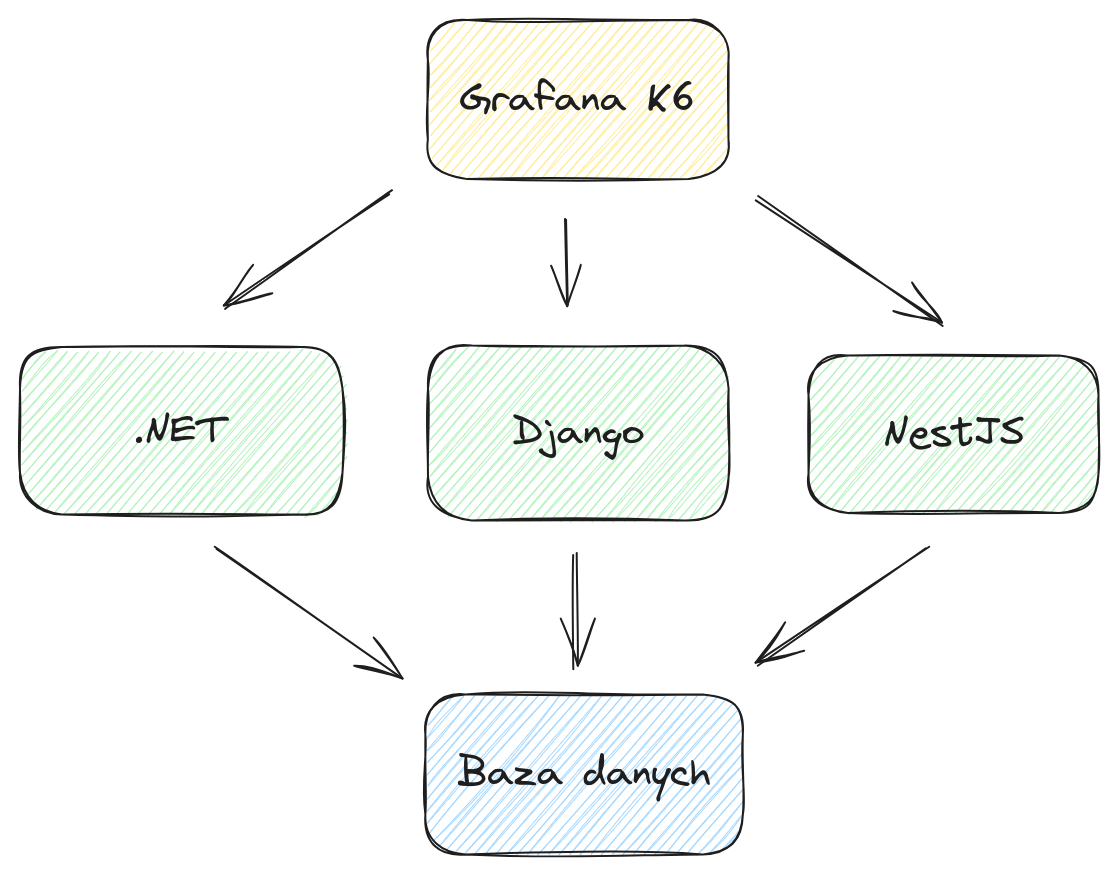
\includegraphics[width=1\linewidth]{rysunki/framework_benchmark_schema.png}
	\caption{Schemat środowiska badawczego}
	\label{rys:docker_schema}
\end{figure}

